%%% LaTeX Template: Curriculum Vitae
%%%
%%% Source: http://www.howtotex.com/
%%% Feel free to distribute this template, but please keep the referal to HowToTeX.com.
%%% Date: July 2011

%%% ------------------------------------------------------------
%%% BEGIN PREAMBLE
%%% ------------------------------------------------------------
\documentclass[paper=a4,fontsize=11pt]{scrartcl}	 			% KOMA-article class
							
%\usepackage[english]{babel}								% English language/hyphenation
%\usepackage[protrusion=true,expansion=true]{microtype}		% Better typography
\usepackage{hyperref}
\usepackage{amsmath,amsfonts,amsthm}					% Math packages
\usepackage[pdftex]{graphicx}								% Enable pdflatex
\usepackage[svgnames]{xcolor}							% Colors by their 'svgnames'
\usepackage{geometry}
	\textheight=700px									% Saving trees ;-) 
\usepackage{url}										% Clickable URL's
\usepackage{wrapfig}									% Wrap text along figures

\frenchspacing									% Better looking spacings after periods
\pagestyle{empty}								% No pagenumbers/headers/footers
%\usepackage{bbding}									% Symbols

%%% Custom sectioning (sectsty package)
%%% ------------------------------------------------------------
\usepackage{sectsty}							% Custom sectioning (see below)

\sectionfont{%									% Change font of \section command
	\usefont{OT1}{phv}{b}{n}%					% bch-b-n: CharterBT-Bold font
	\sectionrule{0pt}{0pt}{-5pt}{3pt}
	}

%%% Macros
%%% ------------------------------------------------------------
\newlength{\spacebox}
\settowidth{\spacebox}{8888888888}				% Box to align text
\newcommand{\sepspace}{\vspace*{1em}}			% Vertical space macro

\newcommand{\MyName}[1]{
		\Huge \usefont{OT1}{phv}{b}{n} \hfill #1 		% Name
		\par \normalsize \normalfont}
		
\newcommand{\MySlogan}[1]{
		\large \usefont{OT1}{phv}{m}{n}\hfill \textit{#1} % Slogan (optional)
		\par \normalsize \normalfont}

\newcommand{\NewPart}[1]{\section*{\uppercase{#1}}}

\newcommand{\PersonalEntry}[2]{
		\noindent\hangindent=2em\hangafter=0 		% Indentation
		\parbox{\spacebox}{						% Box to align text
		\textit{#1}}								% Entry name (birth, address, etc.)
		\hspace{1.5em} #2 \par}					% Entry value

\newcommand{\SkillsEntry}[2]{						% Same as \PersonalEntry
		\noindent\hangindent=2em\hangafter=0 		% Indentation
		\parbox{\spacebox}{						% Box to align text
		\textit{#1}}								% Entry name (birth, address, etc.)
		\hspace{1.5em} #2 \par}					% Entry value	
		
\newcommand{\EducationEntry}[4]{
		\noindent \textbf{#1} \hfill 					% Study
		\colorbox{Black}{%
			\parbox{6.5em}{%
			\hfill\color{White}#2}} \par				% Duration
		\noindent \textit{#3} \par					% School
		\noindent\hangindent=2em\hangafter=0 \small #4 	% Description
		\normalsize \par}

\newcommand{\WorkEntry}[4]{						% Same as \EducationEntry
		\noindent \textbf{#1} \hfill 					% Jobname
		\colorbox{Black}{\color{White}#2} \par		% Duration
		\noindent \textit{#3} \par					% Company
		\noindent\hangindent=2em\hangafter=0 \small #4 	% Description
		\normalsize \par}
		
\newcommand{\BibEntry}[2]{
		\noindent \textbf{#1} \hfill \par					% Study
		\noindent\hangindent=2em\hangafter=0 \small #2 	% Description
		\normalsize \par}
		
		



%%% ------------------------------------------------------------
%%% BEGIN DOCUMENT
%%% ------------------------------------------------------------
\begin{document}
\begin{wrapfigure}{l}{0.5\textwidth}
	\vspace*{-4em}
		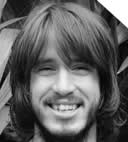
\includegraphics[width=0.2\textwidth]{Doug-Kelley.jpg}
\end{wrapfigure}

\MyName{Douglas Kelley}
\MySlogan{Curriculum Vitae}

\sepspace

%%% Personal details
%%% ------------------------------------------------------------
\NewPart{Personal details}{}

\PersonalEntry{Birth}{6\textsuperscript{th} August, 1984} 
\PersonalEntry{Address}{6/1 Tasman Pl. Macquarie Park, NSW, Australia, 2113}
\PersonalEntry{Phone}{+61 (0) 468790426}
\PersonalEntry{Mail}{\url{douglas.kelley@mq.edu.au}}

%%% Education
%%% ------------------------------------------------------------
\NewPart{Education}{} 

\EducationEntry{\href{http://bcd.mq.edu.au/?page_id=171}{Ph.D. Ecology}}{2010-2014}{\href{http://bio.mq.edu.au/}{Biological Science, Macquarie University}}
  {\textbf{\href{http://bcd.mq.edu.au/?p=361}{Modelling Australian fire regimes:}} Benchmarking and developing the LPX Dynamic Global Vegetation Model (DGVM) to improve the simulation of fire and fire-vegetation interacting. Using this new version of LPX to simulate fire, vegetation and carbon dynamics in Australia over the 21\textsuperscript{st} century}
\sepspace

\EducationEntry{\href{http://www.bristol.ac.uk/cabot/postgrad/msc-ccsp.html}
             {MSc. Earth System Science}}{2007-2008}{\href{http://www.bristol.ac.uk/earthsciences/}{Earth Sciences, Bristol University}}
  {\textbf{Main dissertation: Statistical modelling of global fire regimes.} Other subjects covered: Climate change science and policy; Earth system modelling; Natural hazards; Remote sensing \& GIS; Isotopes and other Earth System tracers}
\sepspace

\EducationEntry{\href{http://www2.warwick.ac.uk/study/undergraduate/courses/f300}{BSc. Physics}}{2002-2007}{\href{http://www2.warwick.ac.uk/fac/sci/physics/}{Physics, University of Warwick}}
  {Main dissertation: Modelling atmospheric effects on starlight.}
  
  
\NewPart{Awards}
\EducationEntry{\href{http://www.hdr.mq.edu.au/information_about/scholarships}{International Macquarie University Research \\ Excellence Scholarship (iMQRES)}}{2010-2014} {Macquarie University postgraduate award}{For completion of Ph.D.}
\sepspace

\EducationEntry{\href{http://www.hdr.mq.edu.au/information_for/current_candidates/financial_support}{Post Graduate Research Fund (PGRF)}}{2013} {Macquarie University - Competitive award to enhance postgraduate research experience}{Funding attendance at the 2013 AGU fall conference in order to present DGVM development and future projection of fire regimes and terrestrial carbon stocks under climate change}
\sepspace

\EducationEntry{Biology postgrad conference best presentation}{2011} {Biological Sciences,Macquarie University}{Best presentation out of the departments 78 postgraduate students at the annual post-graduate conference. Awarded for presentation on a vegetation model benchmarking system}
  
\pagebreak  
\NewPart{Publications}

\BibEntry{In Refereed Journals}{\href{http://www.geosci-model-dev-discuss.net/7/931/2014/gmdd-7-931-2014.html}{\textbf{Kelley, D. I.}, Harrison, S. P. and Prentice, I. C.: Improved simulation of fire-vegetation interactions in the Land surface Processes and eXchanges Dynamic Global Vegetation Model (LPX-Mv1), Geoscientific Model Development Discussions, 7(1), 931--1000, 2014.}}


\BibEntry{} {\href{http://onlinelibrary.wiley.com/doi/10.1002/jgrg.20118/abstract}{Kaminski, T., Knorr, W., Sch, G., Scholze, M., Rayner, P. J., Zaehle, S., Blessing, S., Dorigo, W., Gayler, V., Giering, R., Gobron, N., Grant, J. P., Houweling, S., Kato, T., Kattge, J., \textbf{Kelley, D. I.}, Kemp, S., Koffi, E. N., Mathieu, P. P., Pinty, B., Reick, C. H., Vossbeck, M., Widmann, H. and Ziehn, T.: The BETHY / JSBACH Carbon Cycle Data Assimilation System : experiences and challenges, Journal of Geophysical Research, available on-line, 2013.}}


\BibEntry{} {\href{http://www.biogeosciences.net/10/3313/2013/bg-10-3313-2013.html}{\textbf{Kelley, D. I.}, Prentice, I. C., Harrison, S. P., Wang, H., Simard, M., Fisher, J. B. and Willis, K. O.: A comprehensive benchmarking system for evaluating global vegetation models, Biogeosciences, 10(5), 3313--3340, 2013.}}


\BibEntry{} {\href{http://www.nature.com/ngeo/journal/v5/n1/full/ngeo1324.html}{Ciais, P., Tagliabue, A., Cuntz, M., Bopp, L., Scholze, M., Hoffmann, G., Lourantou, A., Harrison, S. P., Prentice, I. C., \textbf{Kelley, D. I.}, Koven, C. and Piao, S. L.: Large inert carbon pool in the terrestrial biosphere during the Last Glacial Maximum, Nature Geoscience, 5(1), 74--79, 2012.}}


\BibEntry{} {\href{http://onlinelibrary.wiley.com/doi/10.1029/2010GB003906/abstract}{Prentice, I. C., \textbf{Kelley, D. I.}, Foster, P. N., Friedlingstein, P., Harrison, S. P. and Bartlein, P. J.: Modelling fire and the terrestrial carbon balance, Global Biogeochemical Cycles, 25(3), 1--13, 2011.}}
\sepspace
%\pagebreak

\BibEntry{Submitted} {Harrison, S. P., \textbf{Kelley, D. I.}, Wang, H., Herbert, A., Li, G., Bradstock, R., Fontaine, J., Enright, N., Murphy, B. P., Penman, T. and Russell-Smith, J.: Patterns in fire-response trait abundances in Australia using a new database of plot-level measurements for fire model evaluation., Global Ecology and Biogeography.}

\BibEntry{} {\textbf{Kelley, D. I.}, Harrison, S. P.: Impact of re-sprouting on future forest survival and carbon stocks in fire-prone ecosystems, Ecological Research Letters}

\BibEntry{} {Zeppel, M., Adams, H., West, A., \textbf{Kelley, D. I.}, Medlyn, B., Fensham, R., Dawson, T., Tissue, D. and Harrison, S.: Drought-induced mortality within resprouters. New Phytologist }


\NewPart{Presentations}
\BibEntry{International conferences} {\textbf{Kelley, D I.}, Harrison, S. P. and Prentice, I. C.: Implications of introducing realistic fire response traits in a Dynamic Global Vegetation Model, AGU Fall Meeting Abstracts, 1,  p.6. Dec 2013.}
\sepspace

\BibEntry{Visits and Internal Presentations} {\textbf{Kelley, D I.}, Harrison, S. P. and Prentice, I. C.: The LPX fire-enabled Vegetation Model, visit to Centre for Environmental Risk Management of Bushfires, University of Wollongong, NSW, Australia. May 2013.}

\BibEntry{} {\textbf{Kelley, D I.}, Harrison, S. P., Prentice, I. C. and Medlyn B. : The effects of climate change on Australian fire regimes, Postgraduate supplementary conference, Macquarie University, Sydney, Australia. Nov 2012.}

\BibEntry{} {\textbf{Kelley, D I.}: Development of lightning ignitions scheme in LPX-DGVM, Biosphere and Climate Dynamics brown bag seminars, Macquarie University, Sydney, Australia. Sep 2012.}

\BibEntry{} {\textbf{Kelley, D I.}: Benchmarking vegetation and fire in LPX-DGVM, Biosphere and Climate Dynamics brown bag seminars, Macquarie University, Sydney, Australia. Mar 2012.}

\BibEntry{} {\textbf{Kelley, D I.}, Prentice, I. C., Wang, H., Wills, K. and Harrison, S. P.: A comprehensive benchmarking system for evaluating global vegetation models, Postgraduate supplementary conference, Macquarie University, Sydney, Australia. Nov 2011.}

\BibEntry{} {\textbf{Kelley, D I.}, Prentice, I. C., Wang, H., Wills, K. and Harrison, S. P.: A comprehensive benchmarking system for evaluating global vegetation models, Climate Futures Postgraduate Forum, Macquarie University, Sydney, Australia. Nov 2011.}


\BibEntry{} {\textbf{Kelley, D I.}: Benchmark data-sets for assessing DGVM performance, Biosphere and Climate Dynamics brown bag seminars, Macquarie University, Sydney, Australia. Sep 2011.}
\BibEntry{} {\textbf{Kelley, D I.}, Harrison, S. P. and Prentice, I. C.: The effects of climate change on Australian fire regimes, Postgraduate supplementary conference, Macquarie University, Sydney, Australia. 17th Nov 2010.}

\BibEntry{} {\textbf{Kelley, D I.}: Transient Biomization Scheme, course seminar for Msc Earth Systems Science, Department of Earth Sciences, University of Bristol, UK. 2 July 2008.}

\BibEntry{} {\textbf{Kelley, D I.}, Elena Counce: Forest Fire simulator, course seminar for Msc Earth Systems Science, Department of Earth Sciences, University of Bristol, UK. 19 Nov 2007.}
\sepspace

\BibEntry{Posters} {\textbf{Kelley, D I.}, Harrison, S. P.: Comparison of simulated fire regimes at the Last Glacial Maximum and for the Mid-Holocene with charcoal data, QUEST: Quantifying and Understanding the Earth System Open Science Conference and Annual Science Meeting, Mar 2008}

\NewPart{Workshops and Consultancy Visits}
\EducationEntry{Using plant functional traits to predict ecosystem vulnerability to changing fire regimes}{May 2013} {Data Synthesis workshop for fire resilience and response traits}{Australian Centre for Ecological Analysis and Synthesis (ACEAS), University of Queensland.}
\sepspace
\pagebreak
\EducationEntry{Fire response traits database}{May 2013} {Workshop on construction of database on distribution of different resprouting traits in climate space, as part of the Australian Centre for Ecological Analysis and Synthesis (ACEAS) Working group 'Using plant functional traits to predict ecosystem vulnerability to changing fire regimes'.}{Macquarie University, Sydney, Australia.}
\sepspace

\EducationEntry{Technical Assistance for Climate Change}{Oct 2009} {Report on Impacts of Future Climate Change on Vegetation, Fire, and Runoff in Jordan, Royal Society for the Conservation of Nature, Jordan}
\sepspace

\NewPart{Training Courses}

\EducationEntry{Software Carpentry}{Feb 2013} {Programming philosophy, code structure and version control}

\EducationEntry{Genses\textit{2}Geoscience: Writing for journals}{Aug 2012} {Drafting and writing journal articles and research proposals}

\EducationEntry{Genses\textit{2}Geoscience: \textsc{sql}}{Sep 2011} {Database Construction using sql}

\EducationEntry{Genses\textit{2}Geoscience: Teaching in small groups}{Aug 2011} {Effective questioning, encouraging equal participation, and managing student  behaviour.}

\EducationEntry{Planning and writing journal articles}{Nov 2009} {Planning articles to fit journals}


%%% Skills
%%% ------------------------------------------------------------
\NewPart{Skills}{}

%\SkillsEntry{Programming Code}{Fortran}
%\SkillsEntry{}{C}
%\SkillsEntry{}{C++} 

\SkillsEntry{Programming}{Fortran, \textsc{C++}, C, Shell, R, \textsc{Python}, \textsc{Matlab}, VB.}
\SkillsEntry{Languages}{\textsc{Git} and svn version control (see \href{https://bitbucket.org/douglask3}{bitbucket.org/douglask3)}} 
\vspace{1cm}
\SkillsEntry{Publishing}{html/css/\textsc{php} (see \href{http://www.eppingdac.com.au/}{www.eppingdac.com.au}), \textsc{MarkDown} \LaTeX, }
\SkillsEntry{Languages/}{GIMP, Scribus, \textsc{Photoshop/Illustrator}}
\SkillsEntry{Software}{plus standard office/open office software}

%%% Work experience
%%% ------------------------------------------------------------
\NewPart{Relevant Work experience}{}

\EducationEntry{Reasearch Assistant}{2008-2010}{\href{http://www.bristol.ac.uk/geography/} {Geographical Sciences, University of Bristol}, Full-time}
  {DGVM fire model development. Applying developed model to: test to effectiveness of different fire management techniques in current and future climates; simulate paleo vegetation and carbon stocks.}
\sepspace
\pagebreak
\EducationEntry{\href{http://www.greencycles.org/greencycles1/ES4\%20flyer\_2008.pdf}{Earth System Science Summer School co-ordinator}}{2008}{Department of Earth Science, Bristol University, Part-time}{Publicity; lecture and seminar timetabling; finding and organising guest lectures; general admin.}
\sepspace 
%

\EducationEntry{Widening Participation}{2008}{\href{http://www.bristol.ac.uk/sraa/wpur-office/}{Widening Participation Office, Bristol University}, Part-time}{Working with students in primary and secondary education to encourage university attendance from low socio-economic backgrounds: helping organize \& run University open days and campus tours; in-school presentations and career evenings.}

\NewPart{Relevant Extra-Circular activity}{}
\EducationEntry{Committee member responsible for Web-design,\\ Communications, and social runners}{2011-present}{\href{http://www.eppingdac.com.au/}{Epping and District Athletics Clubs}}
  {Website development (\href{http://www.eppingdac.com.au/}{www.eppingdac.com.au}); designing, producing and distributing newsletter  (\href{http://www.eppingdac.com.au/newsletter}{www.eppingdac.com.au/newsletter}) and e-publicity for local community running and athletics club}
\sepspace  

\EducationEntry{Student Union involvment}{2002-2008}{\href{http://www.warwicksu.com/}{University and Warwick}/\href{http://www.ubu.org.uk/}{Bristol University}}
  {Sabbatical year sitting on board of directors of Warwick Students Union responsible for the Student Advice and Welfare department; 3 years as charity trustee and 6 years on student council responsible for Science Faculty representation; committee posts on various student run sports clubs and societies including People and Planet, \href{http://tv.warwick.ac.uk/}{Student TV station}, Student Support Groups, and running clubs}
\sepspace  

\BibEntry{Digital Photography and Art}{\href{http://www3.open.ac.uk/study/undergraduate/course/t189.htm}{Open University undergrad course in digital photography and image manipulation}. \\ See \href{http://www.flickr.com/photos/doug\_from\_the\_uk/}{www.flickr.com/photos/doug\_from\_the\_uk}}


%%% References
%%% ------------------------------------------------------------
%\NewPart{References}{}
%Available upon request


%\nocite{*} 
%\bibliographystyle{plain}
%\renewcommand{\bibname}{References}
%\bibliography{my_papers.bib}

\end{document}